\section{Atom yadrosining tuzilishi. Radioaktivlik}


\begin{enumerate}

\item Atom yadrosi qanday zarralardan tashkil topgan?
\begin{enumerate}[label=\Alph*)]
\item neytron va protonlardan.
\item neytron va elektronlardan.
\item elektron va protonlardan.
\item neytronlardan.
\end{enumerate}

\item Qaysi zarralar jufti nuklonlar deb ataladi?
\begin{enumerate}[label=\Alph*)]
\item proton va neytron.
\item elektron va pozitron.
\item elektron va proton.
\item proton va antiproton.
\end{enumerate}

\item Agar atom yadrosida protonlar soni $Z$, neytronlar soni $N$ bo‘lsa, bu yadroning massa soni $A$ qanday bo‘ladi?
\begin{enumerate}[label=\Alph*)]
\item $Z+N$.
\item $N-Z$.
\item $Z-N$.
\item $N$.
\end{enumerate}

\item Atom yadrosida 30 ta proton, 37 ta neytron bor. Yadro nechta elementar zaryadga ega?
\begin{enumerate}[label=\Alph*)]
\item 7.
\item 37.
\item 30.
\item 67.
\end{enumerate}

\item Mendeleev davriy sistemasidagi tartib raqami 92, tarkibidagi neytronlar soni 146 ta bo‘lgan yadroning massa soni qanday?
\begin{enumerate}[label=\Alph*)]
\item 92.
\item 238.
\item 330.
\item 146.
\end{enumerate}

\item Poloniy $^{210}_{84}\text{Po}$ yadrosida nechta proton bor?
\begin{enumerate}[label=\Alph*)]
\item 84.
\item 126.
\item 136.
\item 210.
\end{enumerate}

\item Kislorod $^{17}_8\text{O}$ izotopida nechta nuklon bor?
\begin{enumerate}[label=\Alph*)]
\item 8.
\item 9.
\item 17.
\item 25.
\end{enumerate}

\item $^{225}_{89}\text{Ac}$ yadrosida nechta neytron bor?
\begin{enumerate}[label=\Alph*)]
\item 89.
\item 136.
\item 226.
\item 314.
\end{enumerate}

\item Uranning Mendeleyev jadvalidagi tartib raqami 92, yadrosining massa soni 238. Uning yadrosida nechta neytron bor?
\begin{enumerate}[label=\Alph*)]
\item 92.
\item 143.
\item 146.
\item 238.
\end{enumerate}

\item Neytral atom haqida aytilgan quyidagi fikrlarning qaysilari mutloqo to‘g‘ri?
\begin{itemize}
    \item[I.] Proton va elektronlari soni teng.
    \item[II.] Proton va neytronlari soni teng.
    \item[III.] Neytronlari soni nolga teng.
\end{itemize}
\begin{enumerate}[label=\Alph*)]
\item faqat I.
\item faqat II.
\item faqat III.
\item I va III.
\end{enumerate}

\item Rasmda ko‘rsatilgan ionning zaryadi $+2e$ ga teng. Shu ionning yadro zaryad soni qanday?

\begin{center}
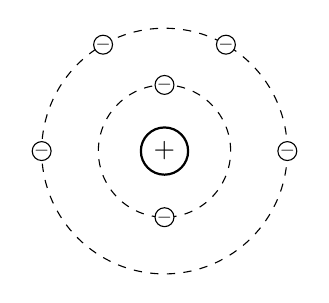
\begin{tikzpicture}[scale=1.2]
  % Nucleus
  \draw[fill=white, thick] (0,0) circle (0.25) node {$+$};
  
  % Orbits
  \draw[dashed, thin] (0,0) circle (0.7);
  \draw[dashed, thin] (0,0) circle (1.3);
  
  % Inner electrons (2)
  \draw[fill=white] (90:0.7) circle (0.1) node[scale=0.7] {$-$};
  \draw[fill=white] (270:0.7) circle (0.1) node[scale=0.7] {$-$};
  
  % Outer electrons (4)
  \draw[fill=white] (60:1.3) circle (0.1) node[scale=0.7] {$-$};
  \draw[fill=white] (120:1.3) circle (0.1) node[scale=0.7] {$-$};
  \draw[fill=white] (0:1.3) circle (0.1) node[scale=0.7] {$-$};
  \draw[fill=white] (180:1.3) circle (0.1) node[scale=0.7] {$-$};
\end{tikzpicture}
\end{center}

\begin{enumerate}[label=\Alph*)]
\item 11.
\item 10.
\item 9.
\item 8.
\end{enumerate}

\item Rasmda keltirilgan atom yadrosining massa soni 17 ga teng. Bu qanday modda atomi?

\begin{center}
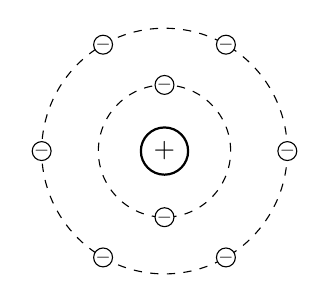
\begin{tikzpicture}[scale=1.2]
  % Nucleus
  \draw[fill=white, thick] (0,0) circle (0.25) node {$+$};
  
  % Orbits
  \draw[dashed, thin] (0,0) circle (0.7);
  \draw[dashed, thin] (0,0) circle (1.3);
  
  % Inner electrons (2)
  \draw[fill=white] (90:0.7) circle (0.1) node[scale=0.7] {$-$};
  \draw[fill=white] (270:0.7) circle (0.1) node[scale=0.7] {$-$};
  
  % Outer electrons (6)
  \draw[fill=white] (0:1.3) circle (0.1) node[scale=0.7] {$-$};
  \draw[fill=white] (60:1.3) circle (0.1) node[scale=0.7] {$-$};
  \draw[fill=white] (120:1.3) circle (0.1) node[scale=0.7] {$-$};
  \draw[fill=white] (180:1.3) circle (0.1) node[scale=0.7] {$-$};
  \draw[fill=white] (240:1.3) circle (0.1) node[scale=0.7] {$-$};
  \draw[fill=white] (300:1.3) circle (0.1) node[scale=0.7] {$-$};
\end{tikzpicture}
\end{center}

\begin{enumerate}[label=\Alph*)]
\item kislorod $^{16}_8\text{O}$.
\item azot $^{14}_7\text{N}$.
\item kislorod izotopi $^{17}_8\text{O}$.
\item ftor $^{19}_9\text{F}$.
\end{enumerate}

\item $^{31}_{15}\text{P}$ izotopi yadrosining zaryadi nimaga teng (C)?
\begin{enumerate}[label=\Alph*)]
\item $2,56\cdot 10^{-18}$.
\item $2,4\cdot 10^{-18}$.
\item $4,96\cdot 10^{-19}$.
\item $2,56\cdot 10^{-19}$.
\end{enumerate}

\item Radioaktivlik bu ayrim atom yadrolarining ...
\begin{enumerate}[label=\Alph*)]
\item Sun’iy parchalanish natijasida faqat radiy atomi yadrosiga aylanishidir.
\item faqat yuqori harorat sharoitida o‘zidan katta energiyali nurlarni chiqarish xususiyatidir.
\item o‘zidan zarrachalar chiqarish bilan o‘z-o‘zidan boshqa yadrolarga aylanish xususiyatidir.
\item o‘zidan issiqlik nurlarini to‘xtovsiz chiqarib turishidir.
\end{enumerate}

\item Quyida sanab o‘tilgan olimlardan qaysi biri radioaktivlikni kashf etgan?
\begin{enumerate}[label=\Alph*)]
\item Pyer Kyuri va Mariya Sklodovskaya-Kyuri.
\item Ernest Rezerford.
\item Antuan Anri Bekkerel.
\item Jeyms Chedvik.
\end{enumerate}

\item $\gamma$-nurlanish nima?
\begin{enumerate}[label=\Alph*)]
\item ionlar oqimi.
\item elektromagnit to‘lqin.
\item protonlar oqimi.
\item elektronlar oqimi.
\end{enumerate}

\item $\beta$-nurlanish nima?
\begin{enumerate}[label=\Alph*)]
\item protonlar oqimi.
\item elektronlar oqimi.
\item elektromagnit to‘lqinlar.
\item neytronlar oqimi.
\end{enumerate}

\item Radioaktiv atom yadrosi ikkita neytron va ikkita protondan iborat zarrani chiqardi. Bu qanday radioaktivlikka kiradi?
\begin{enumerate}[label=\Alph*)]
\item beta.
\item gamma.
\item pozitronli.
\item alfa.
\end{enumerate}

\item Mendeleev jadvalidagi tartib nomeri $Z$ bo‘lgan element yadrosining $\alpha$-yemirilishi natijasida hosil bo‘ladigan elementning tartib nomeri qanday?
\begin{enumerate}[label=\Alph*)]
\item $Z-1$.
\item $Z-2$.
\item $Z$.
\item $Z+2$.
\end{enumerate}

\item Radiy $^{226}_{88}\text{Ra}$ ning $\alpha$-yemirilishi qaysi javobda to‘g‘ri ko‘rsatilgan?
\begin{enumerate}[label=\Alph*)]
\item $^{226}_{88}\text{Ra} \rightarrow ^{210}_{84}\text{Po} + ^4_2\text{He}$.
\item $^{226}_{88}\text{Ra} \rightarrow ^{209}_{83}\text{Bi} + ^4_2\text{He}$.
\item $^{226}_{88}\text{Ra} \rightarrow ^{197}_{79}\text{Au} + ^4_2\text{He}$.
\item $^{226}_{88}\text{Ra} \rightarrow ^{222}_{86}\text{Rn} + ^4_2\text{He}$.
\end{enumerate}

\item $\alpha$-yemirilish natijasida yadro massasi...
\begin{enumerate}[label=\Alph*)]
\item $2\text{ u}$ ga kamayadi, zaryadi $2e$ ga kamayadi.
\item $4\text{ u}$ ga kamayadi, zaryadi $2e$ ga ortadi.
\item deyarli o‘zgarmaydi, zaryadi $2e$ ga kamayadi.
\item $4\text{ u}$ ga kamayadi, zaryadi esa $2e$ ga kamayadi.
\end{enumerate}

\item $\alpha$-yemirilishda yadro qanday o‘zgaradi?
\begin{enumerate}[label=\Alph*)]
\item $-e$ zaryad yo‘qotadi, massasi o‘zgarmaydi.
\item $-2e$ zaryad yo‘qotadi, massasi $2\text{ u}$ ga ortadi.
\item $+e$ zaryad yo‘qotadi, massasi $4\text{ u}$ ga kamayadi.
\item $+2e$ zaryad yo‘qotadi, massasi $4\text{ u}$ ga kamayadi.
\end{enumerate}

\item Qanday radioaktiv yemirilish natijasida toriy $^{232}_{90}\text{Th}$ radiy $^{228}_{88}\text{Ra}$ ga aylanadi?
\begin{enumerate}[label=\Alph*)]
\item $\alpha$.
\item $\beta$.
\item proton bilan nurlantirilganda.
\item $\gamma$.
\end{enumerate}

\item Yadroda proton neytronga aylandi. Bunda yadrodan antineytrino va yana bir zarra ajralib chiqdi. Bu qanday zarra ekanligini aniqlang.
\begin{enumerate}[label=\Alph*)]
\item elektron.
\item pozitron.
\item $\alpha$-zarra.
\item kvant.
\end{enumerate}

\item Keltirilgan yadro reaksiyalarining qaysi biri yadroda pozitronning paydo bo‘lish jarayonini ifodalaydi?
\begin{enumerate}[label=\Alph*)]
\item $^1_1\text{H} + ^1_0\text{n} \rightarrow \text{ }_{+1}\text{e}$.
\item $^1_1\text{p} \rightarrow ^1_0\text{n} + \text{ }_{+1}\text{e} + \tilde{\nu}$.
\item $^1_1\text{H} + ^1_0\text{n} \rightarrow \text{ }_{+1}\text{e} + \gamma$.
\item $^1_1\text{H} + \text{ }_{+1}\text{e} = 2\gamma$.
\end{enumerate}

\item Ketma-ket keladigan ikkita $\alpha$-yemirilishdan so‘ng yadrodagi protonlar soni...
\begin{enumerate}[label=\Alph*)]
\item ikkitaga kamayadi.
\item uchtaga kamayadi.
\item o‘zgarmaydi.
\item to‘rttaga kamayadi.
\end{enumerate}

\item Ketma-ket uchta $\alpha$-yemirilishdan so‘ng $^{234}_{90}\text{Th}$ (toriy izotopi) nimaga aylanadi?
\begin{enumerate}[label=\Alph*)]
\item $^{222}_{84}\text{Po}$.
\item $^{210}_{81}\text{Te}$.
\item $^{238}_{92}\text{U}$.
\item $^{234}_{92}\text{U}$.
\end{enumerate}

\item Ma’lum bir element davriy tizim boshiga qarab 5 ta katakka siljishi uchun nechta $\alpha$ va $\beta$ yemirilish bo‘lishi kerak?
\begin{enumerate}[label=\Alph*)]
\item $2\alpha$ va $3\beta$.
\item $2\alpha$ va $1\beta$.
\item $3\alpha$ va $1\beta$.
\item $3\alpha$ va $2\beta$.
\end{enumerate}

\item Uran $^{235}_{92}\text{U}$ qanday radioaktiv yemirilishdan so‘ng toriy $^{227}_{90}\text{Th}$ ga aylanadi?
\begin{enumerate}[label=\Alph*)]
\item $\alpha$.
\item 2 ta $\alpha$, 2 ta $\beta$.
\item $\alpha$ va $\beta$.
\item $\beta$.
\end{enumerate}

\item Agar yadro $\gamma$-kvant nurlasa, moddani tavsiflovchi qanday kattalik o‘zgaradi?
\begin{enumerate}[label=\Alph*)]
\item atom massasi $\gamma$-kvant massasicha kamayadi.
\item moddaning massa soni o‘zgaradi.
\item atom massasi $\gamma$-kvant massasicha ortadi.
\item moddaning tartib raqami ortadi.
\end{enumerate}

\end{enumerate}



\begin{table}[!ht]
\centering
\begin{tabular}{|c|c|c|c|c|c|c|c|c|c|c|}
\hline
1a & 2a & 3a & 4d & 5b & 6a & 7c & 8b & 9c & 10a & 11d \\ \hline
12c & 13b & 14c & 15c & 16b & 17b & 18d & 19b & 20d & 21d & 22d \\ \hline
23a & 24b & 25b & 26d & 27a & 28c & 29b & 30a & & & \\ \hline
\end{tabular}
\end{table}